\section{Scaling Performances}
\label{sec:scaling}

\begin{figure*}%[ht]
%  \vskip -0.5cm 
  \begin{center}
    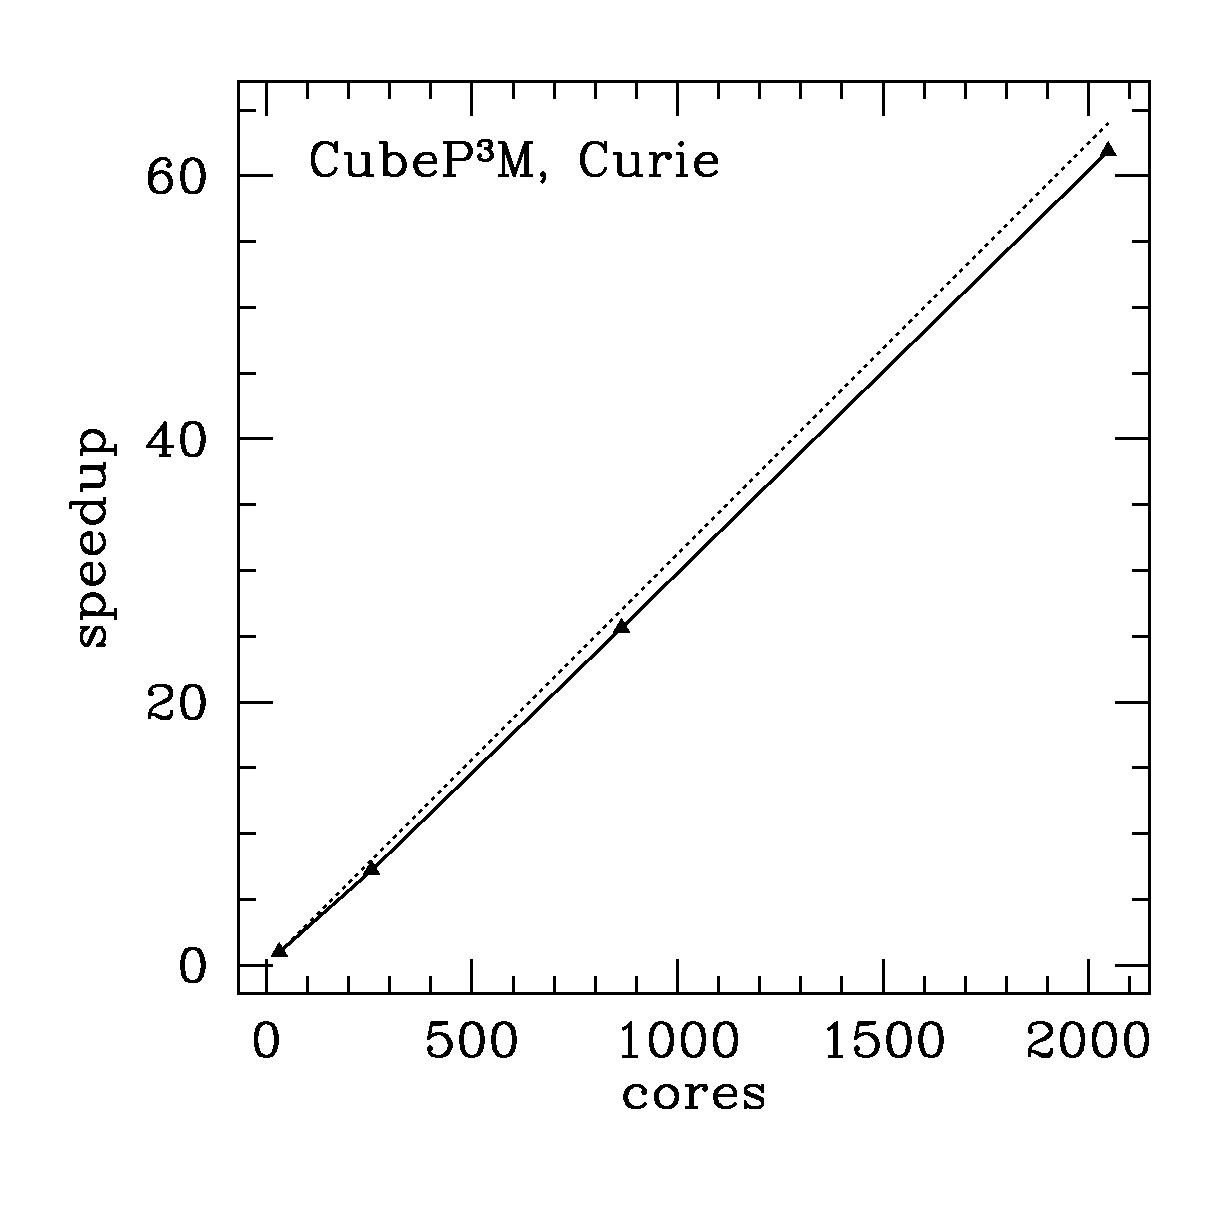
\includegraphics[width=3.2in]{graphs/scaling_cubep3m_curie.eps}
    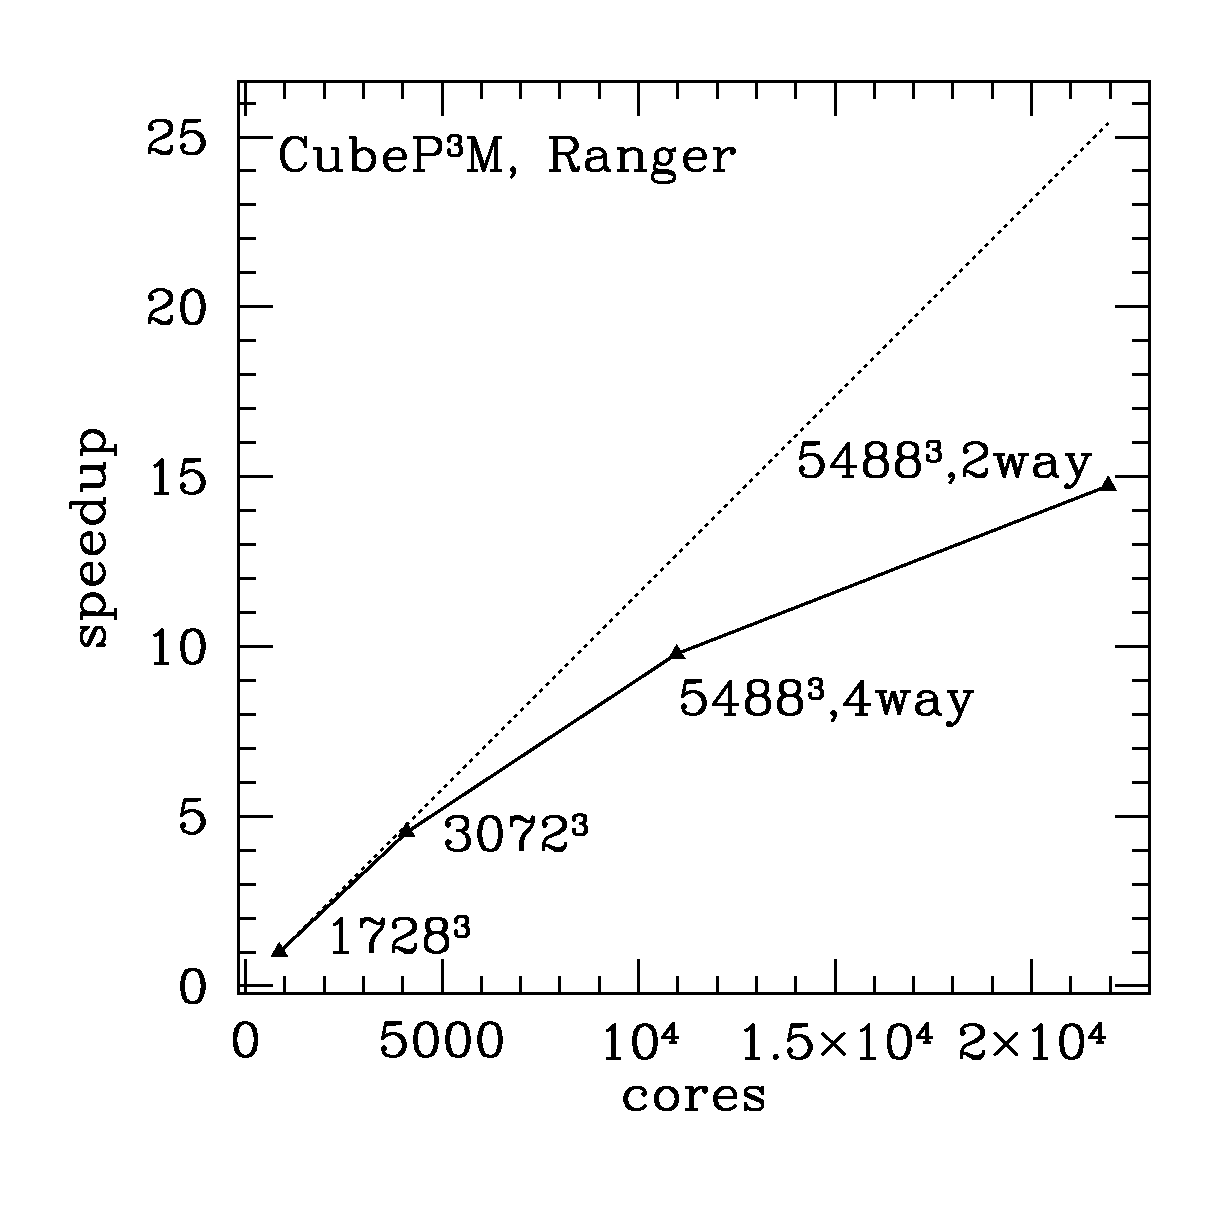
\includegraphics[width=3.2in]{graphs/scaling_cubep3m_new.eps}
%  \vskip -1.2cm 
%  \vskip -0.5cm 
  \caption{Scaling of {\small CUBEP3M} on Curie fat nodes (left) and 
    on Ranger TACC facility for very large number of cores (right). Plotted is the code speedup 
    ($N_{\rm particles}^3/t_{\rm wallclock}$) against core count, normalized by the smallest run 
    in each case. Dashed line indicates the ideal weak 
    scaling. The data are listed in Table \ref{summary_scaling_table}.
    \label{scaling}
% \vskip -0.9cm 
}
\end{center}
\end{figure*}

\begin{table*}%[ht]
  \vskip -0.5cm 
  \begin{center}
\caption{Scaling of {\small CUBEP3M} on Curie. Speedup is 
scaled to the smallest run.}
\label{summary_scaling_table}
\begin{tabular}{@{}|llllll|}
\hline
number of cores & speedup & ideal speedup & absolute timing (min) & 
$N_{\rm particles}$& box size ($h^{-1}$Mpc)
\\[2mm]\hline
%\hline
32  &  1.00 & - &3.2 & $256^3$ & 256\\
256  & 7.21 & 8 &3.55 & $512^3$  & 512\\
864  & 25.63 & 27 &4.8 & $864^3$  & 864\\
2048  & 61.87 & 64 &26.48 & $2048^3$ & 2048 \\
\hline
\end{tabular}
\caption{Scaling of  {\small CUBEP3M} on Ranger. Speedup is scaled to the smallest run.}
\label{summary_scaling_table2}
\begin{tabular}{@{}|llllll|}
\hline
number of cores & speedup & ideal speedup & absolute timing (min) & 
$N_{\rm particles}$& box size ($h^{-1}$Mpc)
\\[2mm]\hline
%\hline
864    & 1.00  & -    &258   & $1728^3$  & 6.3\\
4096   & 4.53  & 4.74 &320   & $3072^3$  & 11.4\\
10976  & 9.78  & 12.7 &845   & $5488^3$  & 20\\
21952  & 14.73 & 25.4 &561   & $5488^3$  & 20 \\
\hline
\end{tabular}
\end{center}
  \vskip -0.7cm 
\end{table*}

%the Ranger system at the Texas Supercomputing
%Center (in top 20 in the world) which is a SunBlade x6420 
%with AMD x86\_64 Opteron Quad Core 2300 MHz (9.2 GFlops)
% ``Barcelona'' processors and Infiniband networking. It has 
%a total of 62976 computing cores and 125952 GB of total 
%memory. Its nodes consist of 4 Quad Core processors and 32 GB 
%of shared RAM. For efficiency reasons (local memory access) we 
%typically use smaller MPI 'nodes' consisting of one Quad Core 
%processor and 8 GB of RAM. 

The parallel algorithm of {\small CUBEP3M} is designed for `weak' 
scaling, i.e. if the number of cores and the problem size 
increase in proportion to each other, then for ideal scaling the 
wall-clock time should remain the same. This is to be in contrasted with `strong' 
scaling codes, whereby the same problem solved on more cores should take 
proportionately less wall-clock time. This weak scaling requirement 
is dictated by the problems we are typically investigating (very 
large and computationally-intensive) and our goals, which are to 
address such large problems in the most efficient way, rather than 
for the least wall-clock time. Furthermore, we recall that there is no explicit 
load balancing feature, thus the code is maximally efficient when the sub-domains
contain roughly an  number of particles. This is true for most
cosmological-size volumes that do not resolve too deep in the non-linear regime, 
but not for e.g. simulations of a single highly-resolved galaxy. 

Because of the volumetric decomposition, the total number of {\small MPI} processes needs
to be a perfect cube. Also, for maximal resource usage, the number of tiles per node 
should be a multiple of the number of available {\small CPU}s per {\small MPI} process,
such that no core sits idle in the threaded block.
Given the available freedom in the parallel configuration, as long as the load is balanced, it is generally good practice to maximize the number of {\small OPENMP} threads and minimize the number of {\small MPI} processes:
the information exchange between cores that are part of the same motherboard is generally much faster.
In addition, having fewer {\small MPI} processes reduces the total amount of buffer zones, 
freeing memory that can be used to increase the mesh resolution. 
As one probes deeper into the non-linear regime however, 
the formation of dense objects can cause memory problems in such configurations, and increasing 
the number of {\small MPI} processes helps to ensure memory locality,
especially in non-uniform memory access (NUMA) environments.


%Since the current Curie is using Intel Nehalem architecture, while 
%the thin Curie nodes will use the newer Westermere Intel architecture, 
%we also show the scaling of our code on the Westermere-based Lonestar 
%computer at the Texas Advanced Computing Centre 


 The intermediary version of the code -- {\small CUBEPM} --
was first  ported to the IBM Blue Gene/L platform, and achieved 
weak-scaling up to 4096 processes (over a billion particles), with the N-body calculation only incurring a 10 per cent overhead 
at runtime (compared to 8 processes) for a balanced workload {\bf (How do we cite Hugh's work on blue gene?)}.  In order to 
accommodate the limited amount of memory available per processing core on the 
Blue Gene/L platform machines, it was necessary to perform the long range {\small MPI FFT}
with a volumetric decomposition \citep{3DFFT}.
Slab decomposition would have required a volume too large to fit in system 
memory given the constraints in the simulation geometry. 

 
The scaling of {\small CUBEP3M}  was first  tested with a dedicated series 
of simulations -- the CURIE simulation suite-- by increasing the size and number of cores on the `fat' 
(i.e. large-memory) nodes of the  Curie supercomputer at the Tr\`{e}s Grand Centre de Calcul (TGCC) in France. 
 For appropriate direct comparison,
all these simulations were performed using the same particle mass 
($M_{\rm particle}=1.07\times10^{11}M_\odot$) and force resolution 
(softening length 50 $h^{-1}$kpc). The box sizes used range from 256 $h^{-1}$Mpc
to 2048 $h^{-1}$Mpc, and the number of particles from $256^3$ to $2048^3$.
Simulations were run on 32 up to 2048 computing cores, also starting from 
redshift $z=100$, and evolving until $z=0$. Our results are shown in Fig. \ref{scaling} and in Table \ref{summary_scaling_table}, and present excellent scaling, within 
$\sim3$ per cent of ideal, at least for up to 2048 cores. 



We have also ran {\small CUBEP3M} on a much larger number of cores, 
from 8000 to up to 21,976, with $5488^3$-$6000^3$ (165 to 216 billion) 
particles on Ranger and on JUROPA at the J\"ulich Supercomputing Centre in Germany, 
which is an Intel Xeon X5570 
(Nehalem-EP) quad-core 2.93 GHz system, also interconnected with Infiniband.
Since it is not practical to perform dedicated scaling tests on such a large number of
computing cores, we instead list in Table \ref{summary_scaling_table2} 
the data directly extracted from production runs. We have found the 
code to scale within 1.5 per cent of ideal up to 4096 cores. 
For larger sizes ($\ge$10,976 cores), the scaling is less ideal,
due to increased communication 
costs, I/O overheads (a single timeslice of $5488^3$ particles is 3.6 TB)
and load balancing issues, but still within $\sim20$ per cent of ideal. 
These first three Ranger runs were performed 
with 4 {\small MPI} processes and 4 threads per Ranger node (`4way')\footnote{For these very large runs, 
we used a NUMA script {\it tacc\_affinity}, specially-provided by the technical staff, 
that bind the memory usage to local sockets, thus ensuring memory affinity. 
This becomes important because the memory sockets per node 
(32 GB RAM/node on Ranger) are actually not equal-access. Generally, the local 
memory of each processor has much shorter access time.}.

Furthermore, due to the increasing clustering of structures at those small 
scales, some of the cuboid sub-domains came to contain a number of particles
well above the 
average, thereby requiring more memory per {\small MPI} process
in order to run until the end. 
As a consequence,  throughout most of their late evolution, the 
largest two of these simulations were run with 4096 and 21,952 cores and 
with only 2 {\small MPI} processes and 8 threads per Ranger node (`2way'), which on 
Ranger allows using up to 16 GB of RAM per {\small MPI} process\footnote{In order to insure 
local memory affinity,  a second special NUMA control script, {\it tacc\_affinity\_2way}, 
was developed for us by the TACC technical staff and allowed to run more efficiently 
in this mode.}. Because each processor accesses memory that is not fully local, this configuration does affect the 
performance somewhat, as does the imperfect load balancing that arises in such situations.
This can be seen in the rightmost point of FIg. \ref{scaling} (right panel), where the scaling 42 per cent below the ideal.
We note that we still get $\sim1.5$ speedup
from doubling the core count, even given these issues. Overall the
code scaling performance is thus satisfactory even at extremely large number of cores.
 We expect the code to handle even larger problems efficiently, and is thus well suited to run on
  next generation Petascale systems. 

Finally, we note that several special fixes had to be developed by  the TACC 
and JUROPA technical staff in order for our largest runs to work properly.
In particular, we encountered unexpected problems from software libraries such as 
{\small MPICH} and {\small FFTW} when applied to calculations of such 
unprecedented size. 

{\bf (We should also compare the memory usage to other codes like Gadget. Ilian mentioned Gadget uses 90 Bytes per particle. Is cubep3m really using 130 Bytes per particle? Check with mem\_usage.)}
